\documentclass[uplatex, titlepage]{jsarticle}
\usepackage[dvipdfmx]{graphicx}
\usepackage{float}

\title{R3.2035年の人口予測と人口問題}
\author{C0118005 A3 秋本 遥基}
\date{}

\begin{document}
\maketitle

\section{目的}

   本レポートでは日本における人口動向について分析を行うとともに、直近にて精度の高いデータを得られている2015年を起点とした人口予測を試みることで、将来における人口動向と、これによって明らかになる人口問題について考察を行うことを目的とした。

\section{方法と結果}

  2015年までの日本の人口の推移の調査、それによる2035年までの男女別及び年齢別人口の予測を行う。調査、分析のために用いたデータは以下に示す。

\begin{itemize}
  \item 国立社会保障・人口問題研究所\cite{source1}
  \item 総務省統計局\cite{source2}
  \item 厚生労働省 \cite{source3}
\end{itemize}

以下は各実験における、数値の分析である。

\subsection{基礎データの導出と分析}

   データより、人口推移についてのグラフを作成した。人口伸び率は$\frac{(今年度人口-前年度人口)}{前年度人口}$により導出した。これを図\ref{fig:graphicx1}に示す。
   また、データから2035年の人口予測をした。これを図\ref{fig:table1}に示す。\\
   この人口予測の手順を示す。前提条件として、データでの差分を生み出さない程度の不用な値(国際移動、年齢不詳)を計算からは除外する。\\
   予測として、前年度から次年度の予測を行う。この際、次年度へ継がれる人口は$生存する確率 \times 前年度の人口$で導出することができる。この生存率は死亡率\cite{source1}から導出する。次に新0歳人口であるが、これは出生率\cite{source1}と前年度の該当年齢人口(15歳以上49歳以下)である女性の数により$出生率 \times 前年度の出産可能人口$で導出される。その際、新0歳人口の男女比は出生比率を元に計算する。女性を100とすると男性の比率は105.5であることより、百分率に直すと男女比率は(男:51.34\%,女:48.66\%)となる。

\begin{figure}[H]
  \centering
    \begin{tabular}{c}
      \begin{minipage}{0.5\hsize}
        \begin{center}
          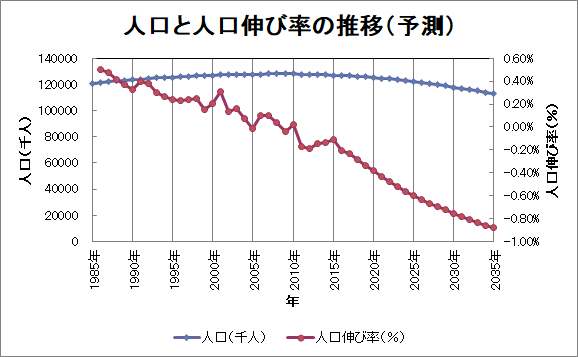
\includegraphics[scale=0.9]{./fffff/f1.png}
          \caption{}
          \label{fig:graphicx1}
        \end{center}
      \end{minipage}
      \begin{minipage}{0.5\hsize}
        \begin{center}
          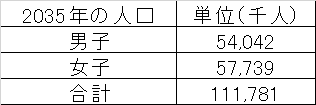
\includegraphics[scale = 0.9]{./fffff/f2.png}
          \caption{}
          \label{fig:table1}
        \end{center}
      \end{minipage}
    \end{tabular}
\end{figure}

また、2015年の出生率と死亡率のグラフをここに示す。

\begin{figure}[H]
  \centering
    \begin{tabular}{c}
      \begin{minipage}{0.5\hsize}
        \begin{center}
          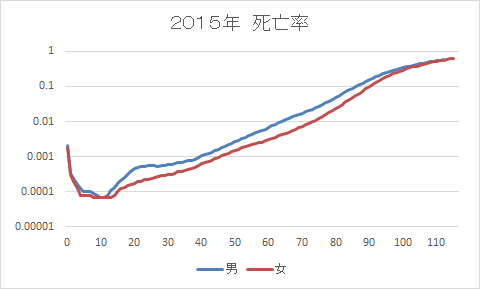
\includegraphics[scale=0.9]{./fffff/ffffff/f8.png}
          \caption{}
          \label{fig:graphicx2}
        \end{center}
      \end{minipage}
      \begin{minipage}{0.5\hsize}
        \begin{center}
          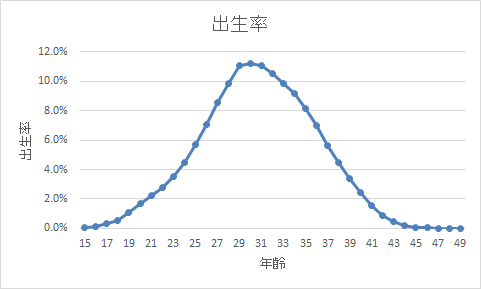
\includegraphics[scale = 0.9]{./fffff/ffffff/f9.png}
          \caption{}
          \label{fig:graphicx3}
        \end{center}
      \end{minipage}
    \end{tabular}
\end{figure}

  結果として人口伸び率推移、図\ref{fig:graphicx1}より異常なほどの人口伸び率の低下が見られることがわかった。短期的兆候として看過するのは難しい予測である。
また、人口の実数値も予測年度以降より平均的な減少傾向を見せている。予想ではあるが長期的に一国の純粋な国民の数がこれほど顕著に減少を見せるのは異常事態であると考える。
死亡率においてはおおよそ、10代後半から男性の方が女性よりも高い数値となっていて、かつ男女どちらも歳を取るごとに数値が高くなる。出生率は30歳前後をピークに数値が下がっている。

\subsection{人口ピラミッドと分析}

次に2015年度の人口ピラミッド図\ref{fig:graphicx5}及び、2035年度の予測人口から人口ピラミッドを作成した。図\ref{fig:graphicx6}

\begin{figure}[H]
  \centering
    \begin{tabular}{c}
      \begin{minipage}{0.5\hsize}
        \begin{center}
          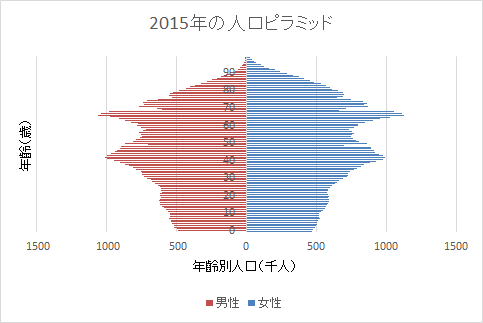
\includegraphics[scale = 0.9]{fffff/f3.png}
          \caption{}
          %\hspace{1.6cm}
          \label{fig:graphicx5}
        \end{center}
      \end{minipage}
      \begin{minipage}{0.5\hsize}
        \begin{center}
          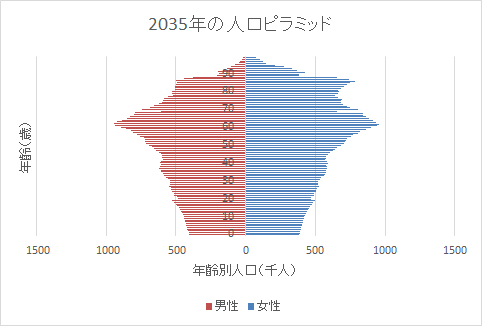
\includegraphics[scale = 0.9]{fffff/f4.png}
          \caption{}
          \label{fig:graphicx6}
        \end{center}
      \end{minipage}
    \end{tabular}
\end{figure}

  結果として、基礎データの導出と同様の様相が見られた。また第一次ベビーブーム世代に当たる男性、女性の高齢者での死亡率の特徴が顕著であり、比較するとやはり男性の方が死亡数が多い。年少人口においては目に見えるほどの減少傾向が見られる。

\subsection{従属人口予想}

  従属人口指数とは扶養者の負担の度合いによる指数であり、$\frac{年少人口 + 老年人口}{生産年齢人口}$により求められる。
  以下に従属人口の推移と、世代別の内訳を示す。

\begin{figure}[H]
  \centering
    \begin{tabular}{c}
      \begin{minipage}{0.5\hsize}
        \centering
          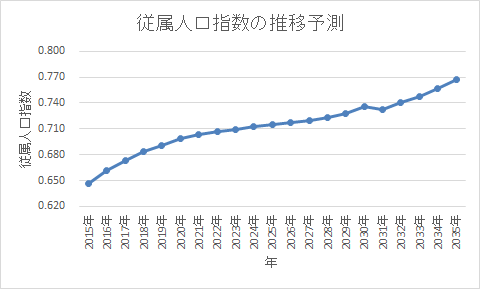
\includegraphics[scale = 0.9]{fffff/f5.png}
          \caption{}
        \label{fig:graphicx7}
      \end{minipage}
      \begin{minipage}{0.5\hsize}
        \centering
          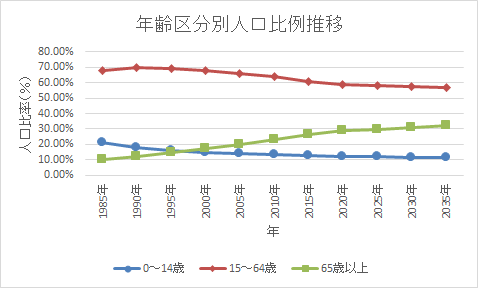
\includegraphics[scale = 0.9]{fffff/f7.png}
          \caption{}
        \label{fig:graphicx8}
      \end{minipage}
  \end{tabular}
\end{figure}

  結果として、従属人口の推移はある時点を除き上昇し続け、内訳から分かるようにその比率において老年人口が大半を占めるように世代がシフトしていることがわかった。
また、その際最も減少しているのが幼年人口であり、社会を存続するのに不安を抱かせる結果であった。

\section{考察}

  目的であった2035年の人口予想であるが、各値(出生率・死亡率)に対してその数値を活かした結果を出すことができた。予想値は2015年以降から始まったが、やはり少しばらつきはあるもののそう合って然るべき値を毎年取り続けていることが理解できた。人が数値に対して任意の気づきを得るのには個々人の恣意性など若干の不明瞭なことが存在しうるとも考えられたが、数値にのみ情報を絞り、測定を行うのがいかに大切か身にしみた。
  死亡率の年代別のグラフ、及び人口ピラミッドより、傾向として存在する数値の関わり合いが予想に対して大きく関わってくるのが大変興味深かった。基礎データの導出の際も述べたが、予想として出される数値であっても、この人口の推移は極めて異常であると思われる。先進国の人口爆発よろしく、国全体に革命的な衛生状況の向上などが起こらない限り人口が一定で増加減少し続けることはありえないと断言しても差し支えない。しかし、実際の予測として本来人口を保つために相互作用され、ぶり返しとして向上されるべき日本の新0歳人口の盛り上がりが全くと言っていいほど見られない。従属人口の数値を鑑みてもこれは社会的にどうしても良いこととは言い切れない。これが果たして現実になってしまうのかは定かではないが、いずれにせよこれに対して何かしらの対応をするのが必要であると思われる。

\begin{thebibliography}{99}
  \bibitem{source1} \verb+http://www.ipss.go.jp+
  \bibitem{source2} \verb+http://www.stat.go.jp/+
  \bibitem{source3} \verb+http://www.mhlw.go.jp+
  \end{thebibliography}
\end{document}
